\section{Analysis of Different Distillation Signal Generated by LLMs}
\label{sec:appendix-A}
Here we provide more details about the prompt design of the \textit{Direct Distillation} experiment.
We also analyze the corresponding generation quality of LLMs, including the stability and interpretability, and compare it with the re-ranking generation.

\subsection{Direct Distillation Prompt Design}
We follow the re-ranking prompt format design and replace the re-ranking task with quantifying the similarity scores of the retrieved documents for LLM's supervised signals generation. An example input prompt and the generated responses without explanations is as follows:\\
\newline
\underline{Input Prompt}:
\begin{verbatim}
I will provide one query with {num} 
documents, each indicated by number 
identifier x. 
Please answer me with a list of the
similarity score between the provided 
query and documents based on your judgment. 
The score should be between 0-1. 
Please don’t use interoperator and only 
output the score list.
<Question> {question} 
<Document1> {document n1} 
...
\end{verbatim}
\underline{Generated Response}:
\begin{verbatim}
[0.1, 0.1, ...., 0.8, 0.2]
\end{verbatim}

\subsection{Comparison with Re-ranking Response}
We compare the responses generated from re-ranking prompts and those derived from similarity score prompts used in the Direct Distillation experiment. 
Specifically, we randomly select 1,000 data instances from the \textit{NQ} dataset, using the queries and their retrieved documents to prompt the LLM to generate both list-wise re-ranking orders and similarity scores.
Examples of responses generated by the LLM, specifically using GPT-4 Turbo, are shown in Table \ref{table:03}.

\begin{figure}[!htbp]
    \centering
    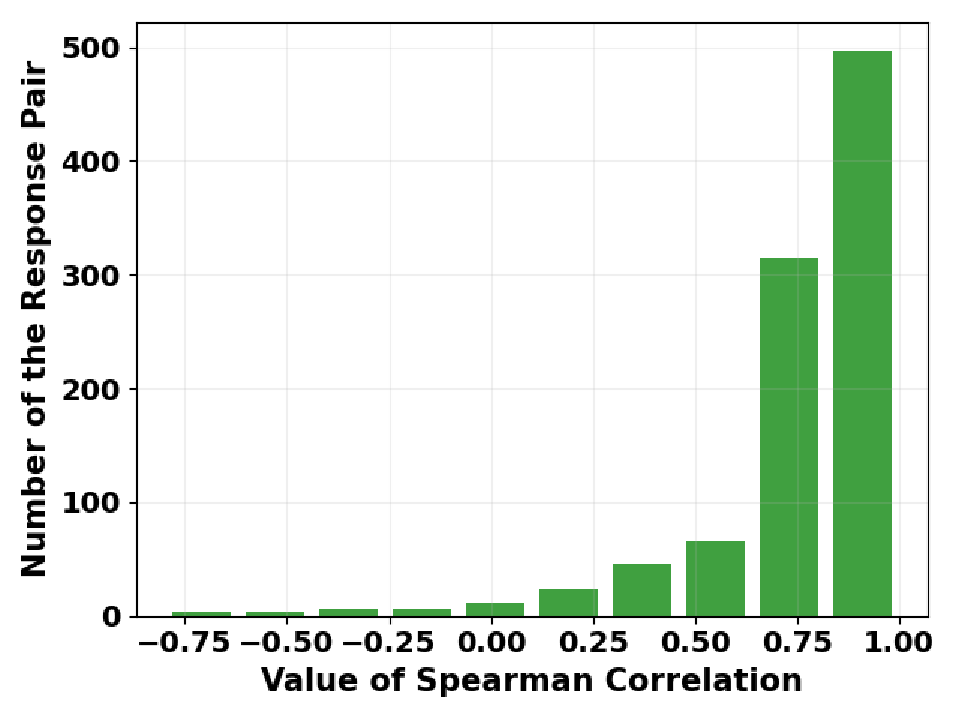
\includegraphics[width=0.48\textwidth]{latex/pic/fig7.pdf}
    \caption{Spearman Correlation between the responses from the re-ranking prompt and the responses from the similarity score prompt.}
    \label{fig:07}
    \vspace{-4mm}
\end{figure}

Table \ref{table:03} shows that responses generated from re-ranking prompts are more interpretable than those from similarity score prompts, which often use scaled values that are ambiguous.
Additionally, responses from the similarity score-based prompt frequently yield extreme values, such as 0.0 (completely dissimilar) or 1.0 (highly similar), in some cases, which means that  that supervision signals based on similarity scores are less informative and act more like binary signals in certain data instances.

Moreover, we use the \textit{Spearman Correlation} to assess the consistency between responses generated from re-ranking prompts and those from similarity score prompts, and the analysis result is visualized in Figure \ref{fig:07}.
A higher Spearman correlation value suggests a stronger positive correlation between the two types of responses.
From Figure \ref{fig:07}, we can see that many response pairs are closely related, indicating the stability and reliability of LLMs in generating responses for similar tasks.
In addition, based on our previous analysis, we can see that the responses from re-ranking prompts are not only reliable but also possess a higher information density compared to those from similarity score prompts, showing that responses from re-ranking prompts have higher-quality supervision capabilities.

\subsection{Implantation Details of Direct Distillation Experiment}
We use the same training settings as those used in Intermediate Distillation experiments.
Superficially, we set the retriever model with a hidden layer size to 768 and initialize it using a dual-encoder Contriever checkpoint.
The model is trained over five epochs using the same dataset as described in Section \ref{sec:4}, with a learning rate of 5e-5, a batch size of 20, and optimization via the Adam optimizer.
In addition, we also limit the size of the relevant document subset $D_n$ to five, and each retrieved document with a maximum length of 128.


\begin{table*}[!ht]
\small
\centering
\begin{tabular}{|p{6cm}|c|p{6cm}|}
\hline
\textbf{Question \& Retrieved Documents} & \textbf{Type} & \multicolumn{1}{c|}{\textbf{LLM's Generation}} \\ 
\hline
\multirow{2}{=}
{\textbf{[Question]} membership in the european union requires countries to have which type of government
\textbf{[Document1] } the european continent. the eu's example is being followed by the african union, the union of south American nations...
\textbf{[Document2] } powers of states, the considerable level of translation and the choice of a lesser city as the capital...
\textbf{[Document3]} principal characteristic of classical {\color{red}democracy}. the concept of a mixed government was studied during the renaissance and the age of reason by niccolo machiavelli, giambattista vico...
\textbf{[Document4]} thus essentially preventing it from participating in government. the european union ( eu ) is an association of twenty - eight sovereign member states...
\textbf{[Document5]} civiletti opinions, not all funding gaps led to shutdowns. of the nine funding gaps between 1980 and 1990, only four led to furloughs...} & \textit{Re-ranking}
& [\textit{Re-ranking order}] {\color{blue}Document5, Document3, Document2, Document1, Document4}.
\textit{[Explanation]} Document5 directly discusses the governmental systems used by most European nations, particularly the parliamentary system, which is relevant since the EU generally comprises nations with parliamentary democracies. This makes it the most relevant to the query about the type of government required for EU membership. Document3 talks about mixed constitutions...\\
\cline{2-3}
& \textit{Similarity Score} & 
[\textit{Similarity scores from Document1 to Document5}] {\color{blue}Doc1:0.0, Doc2:0.1, Doc3:0.3, Doc4:0.1, Doc5:0.7}. 
\textit{[Explanation]} Document1 talks about the EU and various other international organizations, focusing on aspects like the single market and policy integration but does not mention government types required for EU membership. Hence, the score is 0.0. Document2 discusses the structure of EU governance... \\
\hline

\multirow{2}{=}
{{\textbf{[Question]} when was the immigration reform and control act passed}
\textbf{[Document1] } united states temporarily for money or a better life. an increase in legal immigrants migrating to the united states also led to an increase of illegal aliens...
\textbf{[Document2] } there are noted communists, socialists, and anti - american sympathizers. parts of the act remain in place today...
\textbf{[Document3] } ...the immigration reform and control act ( irca ), also known as the simpson 2013 mazzoli act or the reagan amnesty, signed into law by ronald reagan on {\color{red}november 6}, 1986...
\textbf{[Document4] } five percent of the u. s. workforce. it was also estimated that about 70 percent of those illegal workers...
\textbf{[Document5] } to reduce them as restrictionists. "fry traced" restrictions roots " to a surprising surge in illegal and legal immigration...
}
& \textit{Re-ranking} & [\textit{Re-ranking order}] {\color{blue}Document3, Document1, Document4, Document5, Document2}.
\textit{[Explanation]} Document3 directly answers the query by explicitly mentioning the "Immigration Reform and Control Act of 1986" and stating it was signed into law by Ronald Reagan on November 6, 1986. It provides the most specific information related to the query... \\
\cline{2-3}
& \textit{Similarity Score} & [\textit{Similarity scores from Document1 to Document5}] {\color{blue}Doc1:0.0, Doc2:0.0, Doc3:1.0, Doc4:0.0, Doc5:0.0}. 
\textit{[Explanation]} Document1 discusses general immigration trends and issues but does not provide the specific date of the passage of the Immigration Reform and Control Act, which is directly asked in the query. Therefore, it receives a score of 0.0. Although Document2 mentions other immigration-related legislation and acts, it does not specify...\\
\hline

\multirow{2}{=}
{\textbf{[Question]} who sings in there's something about mary  
\textbf{[Document1] } melody. mary described the completed song as "whitney - fied". meron maintains that...
\textbf{[Document2] } ...he film concludes with the two engaging in a kiss while singer / songwriter {\color{red}jonathan richman}, who has periodically narrated the story in song throughout the film...
\textbf{[Document3] } day but her. minutes later bing notices his tackle box has been disturbed, and an instant later the kids see the door to the tent is open...
\textbf{[Document4] } true opinions of other contestants and her stance on the judges. the book achieves in combining fifty years of a'salt of the earth'existence with a new - found life of fame...
\textbf{[Document5] } and breezy number and the narrator opens up the story about bing and his family. and while bing is cleaning the fish, he tells the story of " goldilocks"...
}
& 
\textit{Re-ranking} & [\textit{Re-ranking order}] {\color{blue}Document2, Document5, Document4, Document1, Document3}.
\textit{[Explanation]} Document2 is the most relevant sentence as it directly answers the query. It mentions that Jonathan Richman narrated parts of the story through song throughout the film "There's Something About Mary," which clearly identifies the singer related to your query... \\
\cline{2-3}
& \textit{Similarity Score} & [\textit{Similarity scores from Document1 to Document5}] {\color{blue}Doc1:0.0, Doc2:1.0, Doc3:0.0, Doc4:0.0, Doc5:0.0}. 
\textit{[Explanation]} Document1 discusses a song in a completely different context, related to "Cinderella" and Whitney Houston's music adjustments, not related to the film "There's Something About Mary." Thus, it doesn't answer the query about who sings in the specified film, receives a score of 0.0. Document2 directly answers the query. It mentions that Jonathan Richman narrated parts of the story... \\
\hline    
\end{tabular}
\caption{Examples of two different LLM-generated responses. We also let LLM generate the corresponding explanations in these examples. The red color indicates the corresponding answer to the question.}
\label{table:03}
\end{table*}


% \section{Case Studies of Metric and LLM Distillation in RAG}